\section{Zielsetzung}
\label{sec:Zielsetzung}
Das Ziel des Versuches ist es, das Elastizistätsmodul unterschiedlicher Metallstäbe zu bestimmen.

\section{Theorie}
\label{sec:Theorie}

Kräfte, die auf die Oberfläche eines Objekts einwirken, verursachen Form- und Volumenänderungen. Diese Kräfte werden üblicherweise auf eine Flächeneinheit bezogen und die resultierende physikalische Größe wird als Spannung bezeichnet. 
Die Komponente senkrecht zu ihrer Oberfläche heißt Normalspannung $\sigma$.
Die flächenparallele Komponente ist dagegen die Tangential- oder Schubspannung. 
Ist die Formänderung, die durch die relative Änderung ΔL/L (siehe \autoref{fig:hook}) hervorgerufen wird, klein, so kann mithilfe des Hookeschen Gesetzes eine lineare Beziehung zwischen
der Änderung ΔL/L und der angelegten Spannung $\sigma$ hergestellt werden:
\begin{equation}\label{eq:hook}
    \sigma = E \cdot \frac{\Delta L}{L}.
\end{equation}
Dabei ist $E$ das Elastizistätsmodul und eine Materialkonstante.
\begin{figure}[H]
    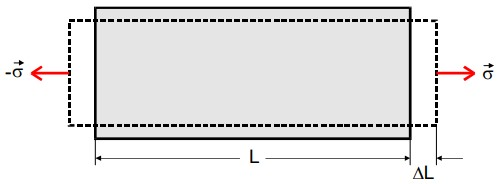
\includegraphics[width=\linewidth]{img/abb1.jpg}
    \caption{Dehnung einer stabförmigen Probe unter dem Einfluss einer Normalspannung.\cite{V103}}
    \label{fig:hook}
\end{figure}
Da die Stauchung oder Streckung bei vielen Materialien nicht einfach herbeizuführen ist, gibt es andere Methoden wie zum Beispiel die 
Biegung zur Bestimmung des Elastizistätsmodul.
Die Biegeverformung lässt sich auf die oben genannte Dehnung zurückführen. Hier ist die Änderung der Querschnittslänge Q der Probe aber nicht mehr konstant. 
Eine stabförmige Probe biegt sich, wenn eine Kraft F auf sie ausgeübt wird, wie in \autoref{fig:biegung} gezeigt.
Die Biegung $D$ ist eine Funktion des Abstands $x$, in der das Elastizistätsmodul $E$ auftritt. Somit kann aus Wertepaaren $D$ und $x$ die Größe $E$ bestimmt werden.
\begin{figure}[H]
    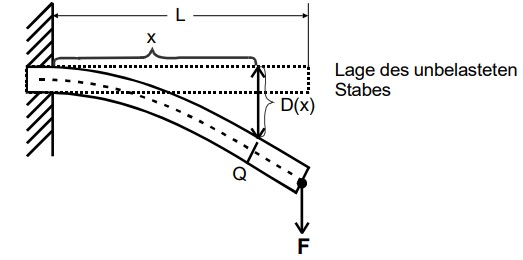
\includegraphics[width=\linewidth]{img/abb2.jpg}
    \caption{Biegung eines elastischen Stabes bei einseitiger Einspannung.\cite{V103}}
    \label{fig:biegung}
\end{figure}
Das Nutzen von Biegeverformungen ist besser im Experiment darstellbar, weil sogar mit kleinen Kräften die Verformung von Körpern herbeizuführen ist.
Die angreifende Kraft erzeugt  ein Drehmoment, wodurch die unteren Körperschichten gestaucht und die oberen gedehnt werden.
In der Mitte tritt daher auch eine neutrale Faser auf, der keine Längenänderung widerfährt.
Als Folge der Verbiegung treten der Kraft entgegengesetzte Normalspannungen auf, d.h. der Stab biegt sich so lange bis sich ein Gleichgewicht zwischen dem
gewichtsbedingten und dem spannungsbedingten Drehmoment einstellt. Dann gilt:
\begin{equation*}
    M_F = M_{\sigma}.
\end{equation*}
$M_{\sigma}$ ist dabei das im inneren auftretende Drehmoment, das sich mithilfe \autoref{fig:msigma} herleiten lässt. Da die Zugspannungen oberhalb der neutralen
Faser und die Druckspannungen unterhalb der neutralen Faser entgegengesetzt, aber betraglich gleich sind, lässt sich das wirkende Drehmoment mit
\begin{equation*}
    M_{\sigma} = \int_{Q} y\sigma(y) dq
\end{equation*}
berechnen.\\
\begin{minipage}[4cm]{0.5\textwidth}
\begin{figure}[H]
    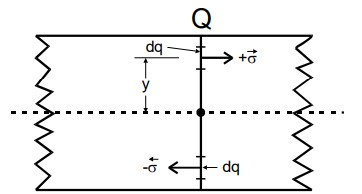
\includegraphics[width=\linewidth]{img/abb3.jpg}
    \caption{Berechnung des inneren \\Drehmoments $M_{\sigma}$.\cite{V103}}
    \label{fig:msigma}
\end{figure}
\vspace{10pt}
\end{minipage}
\begin{minipage}[4cm]{0.5\textwidth}
    Das durch die angreifende Kraft erzeugte Drehmoment, greift mit dem Hebelarm $L-x$ an Q an. Für das äußere Drehmoment ergibt sich also
        \begin{equation*}
            M_F = F \cdot (L-x).
        \end{equation*}
        Die Gleichgewichtslage der Drehmomente ist also 
        \begin{equation*}
            \int_{Q} y\sigma(y) dq = F \cdot (L-x).
        \end{equation*}
        \vspace{10pt}
\end{minipage}
Nach \autoref{eq:hook} ergibt sich für ein kurzes Stabstück $\Delta x$ im Abstand $y$ von der neutralen Faser
\begin{equation*}
    \sigma (y) = E \cdot \frac{\delta x}{\Delta x},
\end{equation*}
wobei $\delta x$ die Längenänderung der Faser ist. Mit geometrischen Überlegungen folgt
\begin{equation}\label{eq:lol}
    E \cdot \frac{d^2 D}{d x^2} I = F \cdot (L-x),
\end{equation}
dabei ist I das Flächenträgheitsmoment, welches sich mit 
\begin{equation}\label{eq:flaeche_traegheit}
    I =  \int_{Q} y^2 dA
\end{equation}
berechnen lässt. Dabei ist das Integral ein Flächenintegral über die Querschnittsfläche des Stabes.
Durch zweimalige Integration von \autoref{eq:lol} ergibt sich die Gleichung für die Auslenkung:
\begin{equation}\label{eq:ausgleich}
    D(x) = \frac{F}{2 \cdot E \cdot I} \biggl(Lx^2 - \frac{x^3}{3}\biggr).
\end{equation}
\\
\\
\begin{minipage}[4cm]{0.45\textwidth}
    \begin{figure}[H]
        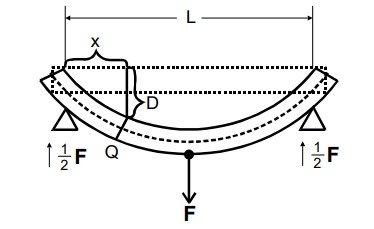
\includegraphics[width=\linewidth]{img/abb4.jpg}
        \caption{Beidseitige Einhängung \\des Stabes.\cite{V103}}
        \label{fig:beidseitig}
    \end{figure}
    \vspace{10pt}
    \end{minipage}
    \begin{minipage}[4cm]{0.55\textwidth}
        Spannt man den Stab auf beiden Seiten ein (\autoref{fig:beidseitig}), so greift die Kraft $F/2$ an der Querschnittsfläche $Q$ an.
        Es gilt daher
        \begin{equation*}
            M_F = 
            \begin{cases}
                -\frac{F}{2}x, & 0 \leq x \leq L/2 \\
                \\
                -\frac{F}{2}(L-x) & L/2 \leq x \leq L.
            \end{cases}
        \end{equation*}
        Setzt man dies in \autoref{eq:lol} ein, lässt sich ein Ausdruck für die Auslenkung finden:
        \begin{equation*}
            D(x) = 
            \begin{cases}
                \frac{F}{48 \cdot E \cdot I} \biggl(-4x^3 + 3L^2x\biggr) & 0 \leq x \leq L/2 \\
                \\
                \frac{F}{48 \cdot E \cdot I} \biggl(4x^3 - 12Lx^2 + 9L^2x - L^3\biggr) & L/2 \leq x \leq L.
            \end{cases}
        \end{equation*}
        \vspace{10pt}
    \end{minipage}
    \newpage